\subsection{Class Diagram}
%Describe here the class diagram of your project
We encountered a challenge with trying to fit the diagram of the project in a single figure, so we divided the original diagram into six smaller, more manageable schemes.
Each of these schemes cover a different scope.

The first one, figure \ref{fig:class-dbentities}, shows the classes that we used to represent data in the business logic layer.
The FullDish, FullOrder and DishIngredient classes are used to describe more complex data objects that do not directly match the entities stored in the database, as they are mainly used to contain data resulting from an SQL JOIN operation.
The cuisine class does not extend the AbstractResource class because we didn't need to express it in JSON format.

All the following diagrams follow the basic REST paradigm that we implemented using a servlet dispatcher for the HTTP requests, some RR(REST Resource) classes for the main logic and DAO(Data Access Object) classes to communicate with the database.
In particular, the second diagram, figure \ref{fig:class-user}, contains all the classes relating to user account operations, like registering, logging-in and logging-out, updating user information and so on.
Also, it shows the different authentication filter classes used on the requests.
The third diagram, figure \ref{fig:class-restaurant}, shows the classes that perform operations relating to the restaurant entity, like creating a restaurant, deleting one or retrieving data about it.
Then the fourth diagram, figure \ref{fig:class-dish}, shows the classes that perform operations relating to the dish entity, like creating a dish, deleting one or retrieving data about it.
The fifth diagram, figure \ref{fig:class-cuisine}, shows the classes that are concerned with listing the cuisine types, which are useful for the advanced search tool.
And lastly, the sixth diagram, in figure \ref{fig:class-order}, shows the classes that perform operations relating to the food ordering process, like displaying the cart, adding dishes to the order, removing them or changing their quantity in the cart.



%Class diagram of db entities classes that represent data to be retrieved or submitted
\begin{center}
    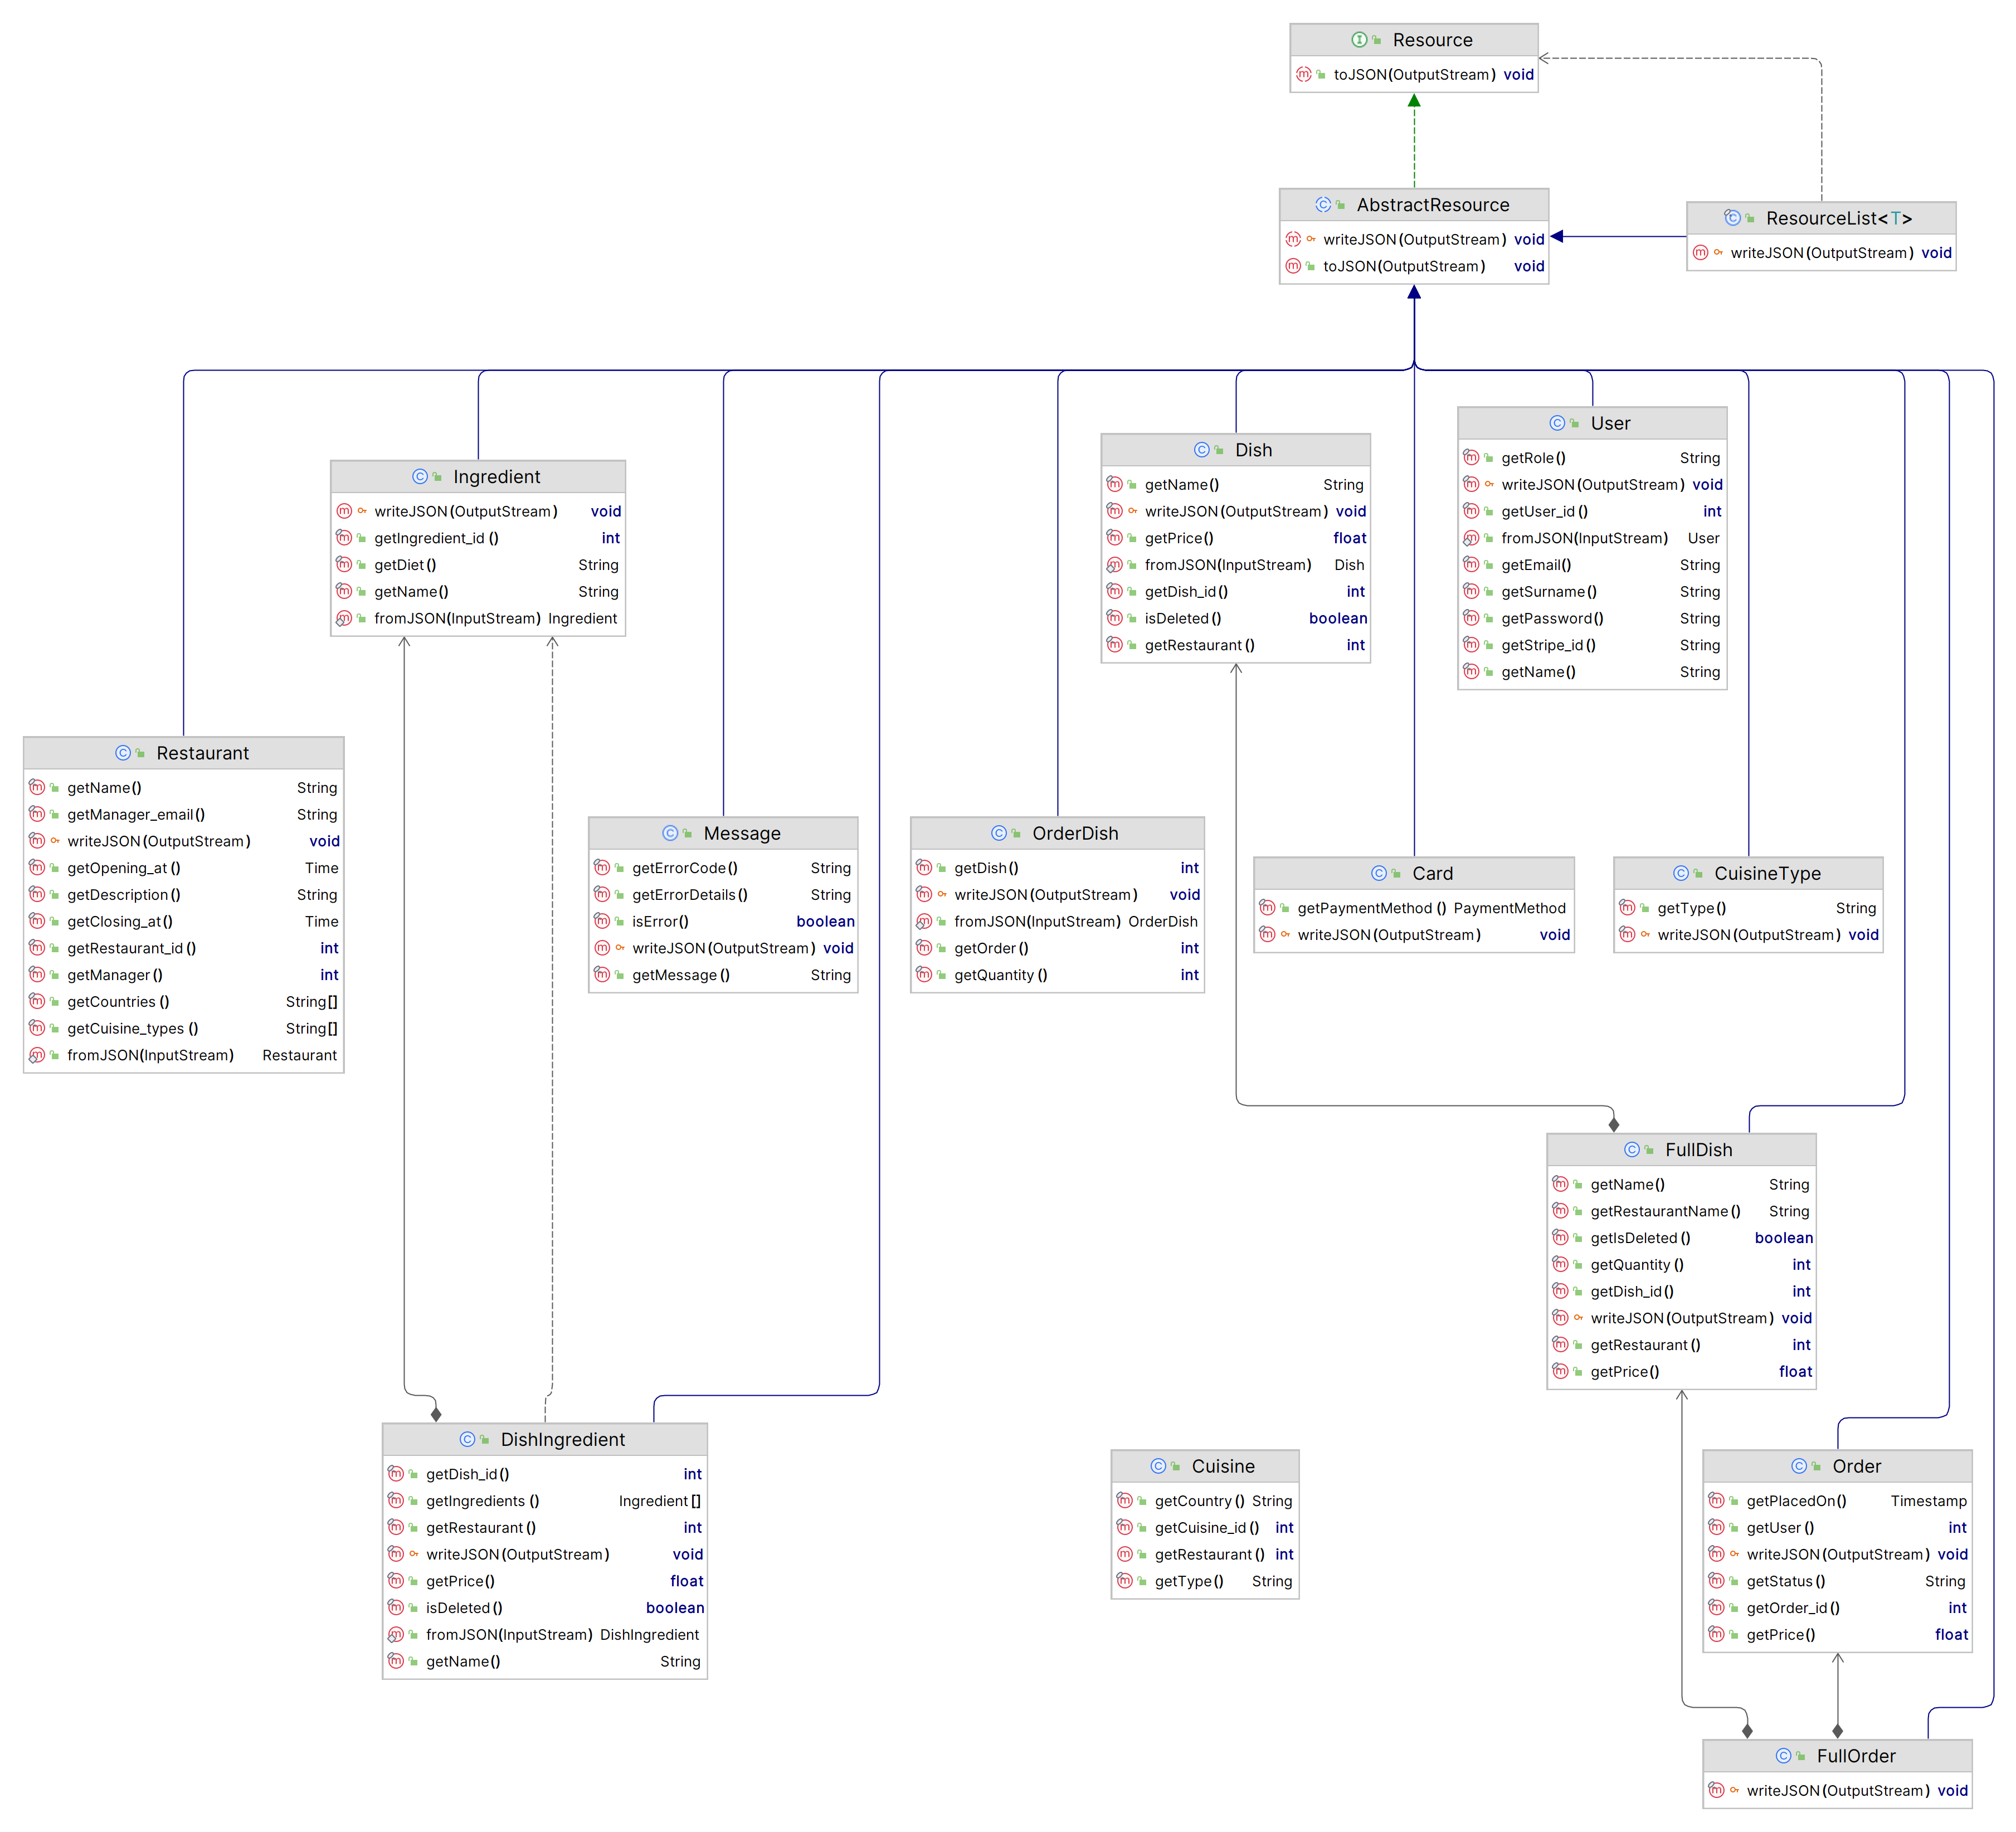
\includegraphics[width=1.0\textwidth]{resources/class-diagrams/dbentities_class_diagram}
    \captionof{figure}{Class diagram of the database entities and their hierarchy.}
    \label{fig:class-dbentities}
\end{center}


%Class diagram of the user REST classes and filters for authentication
\begin{center}
    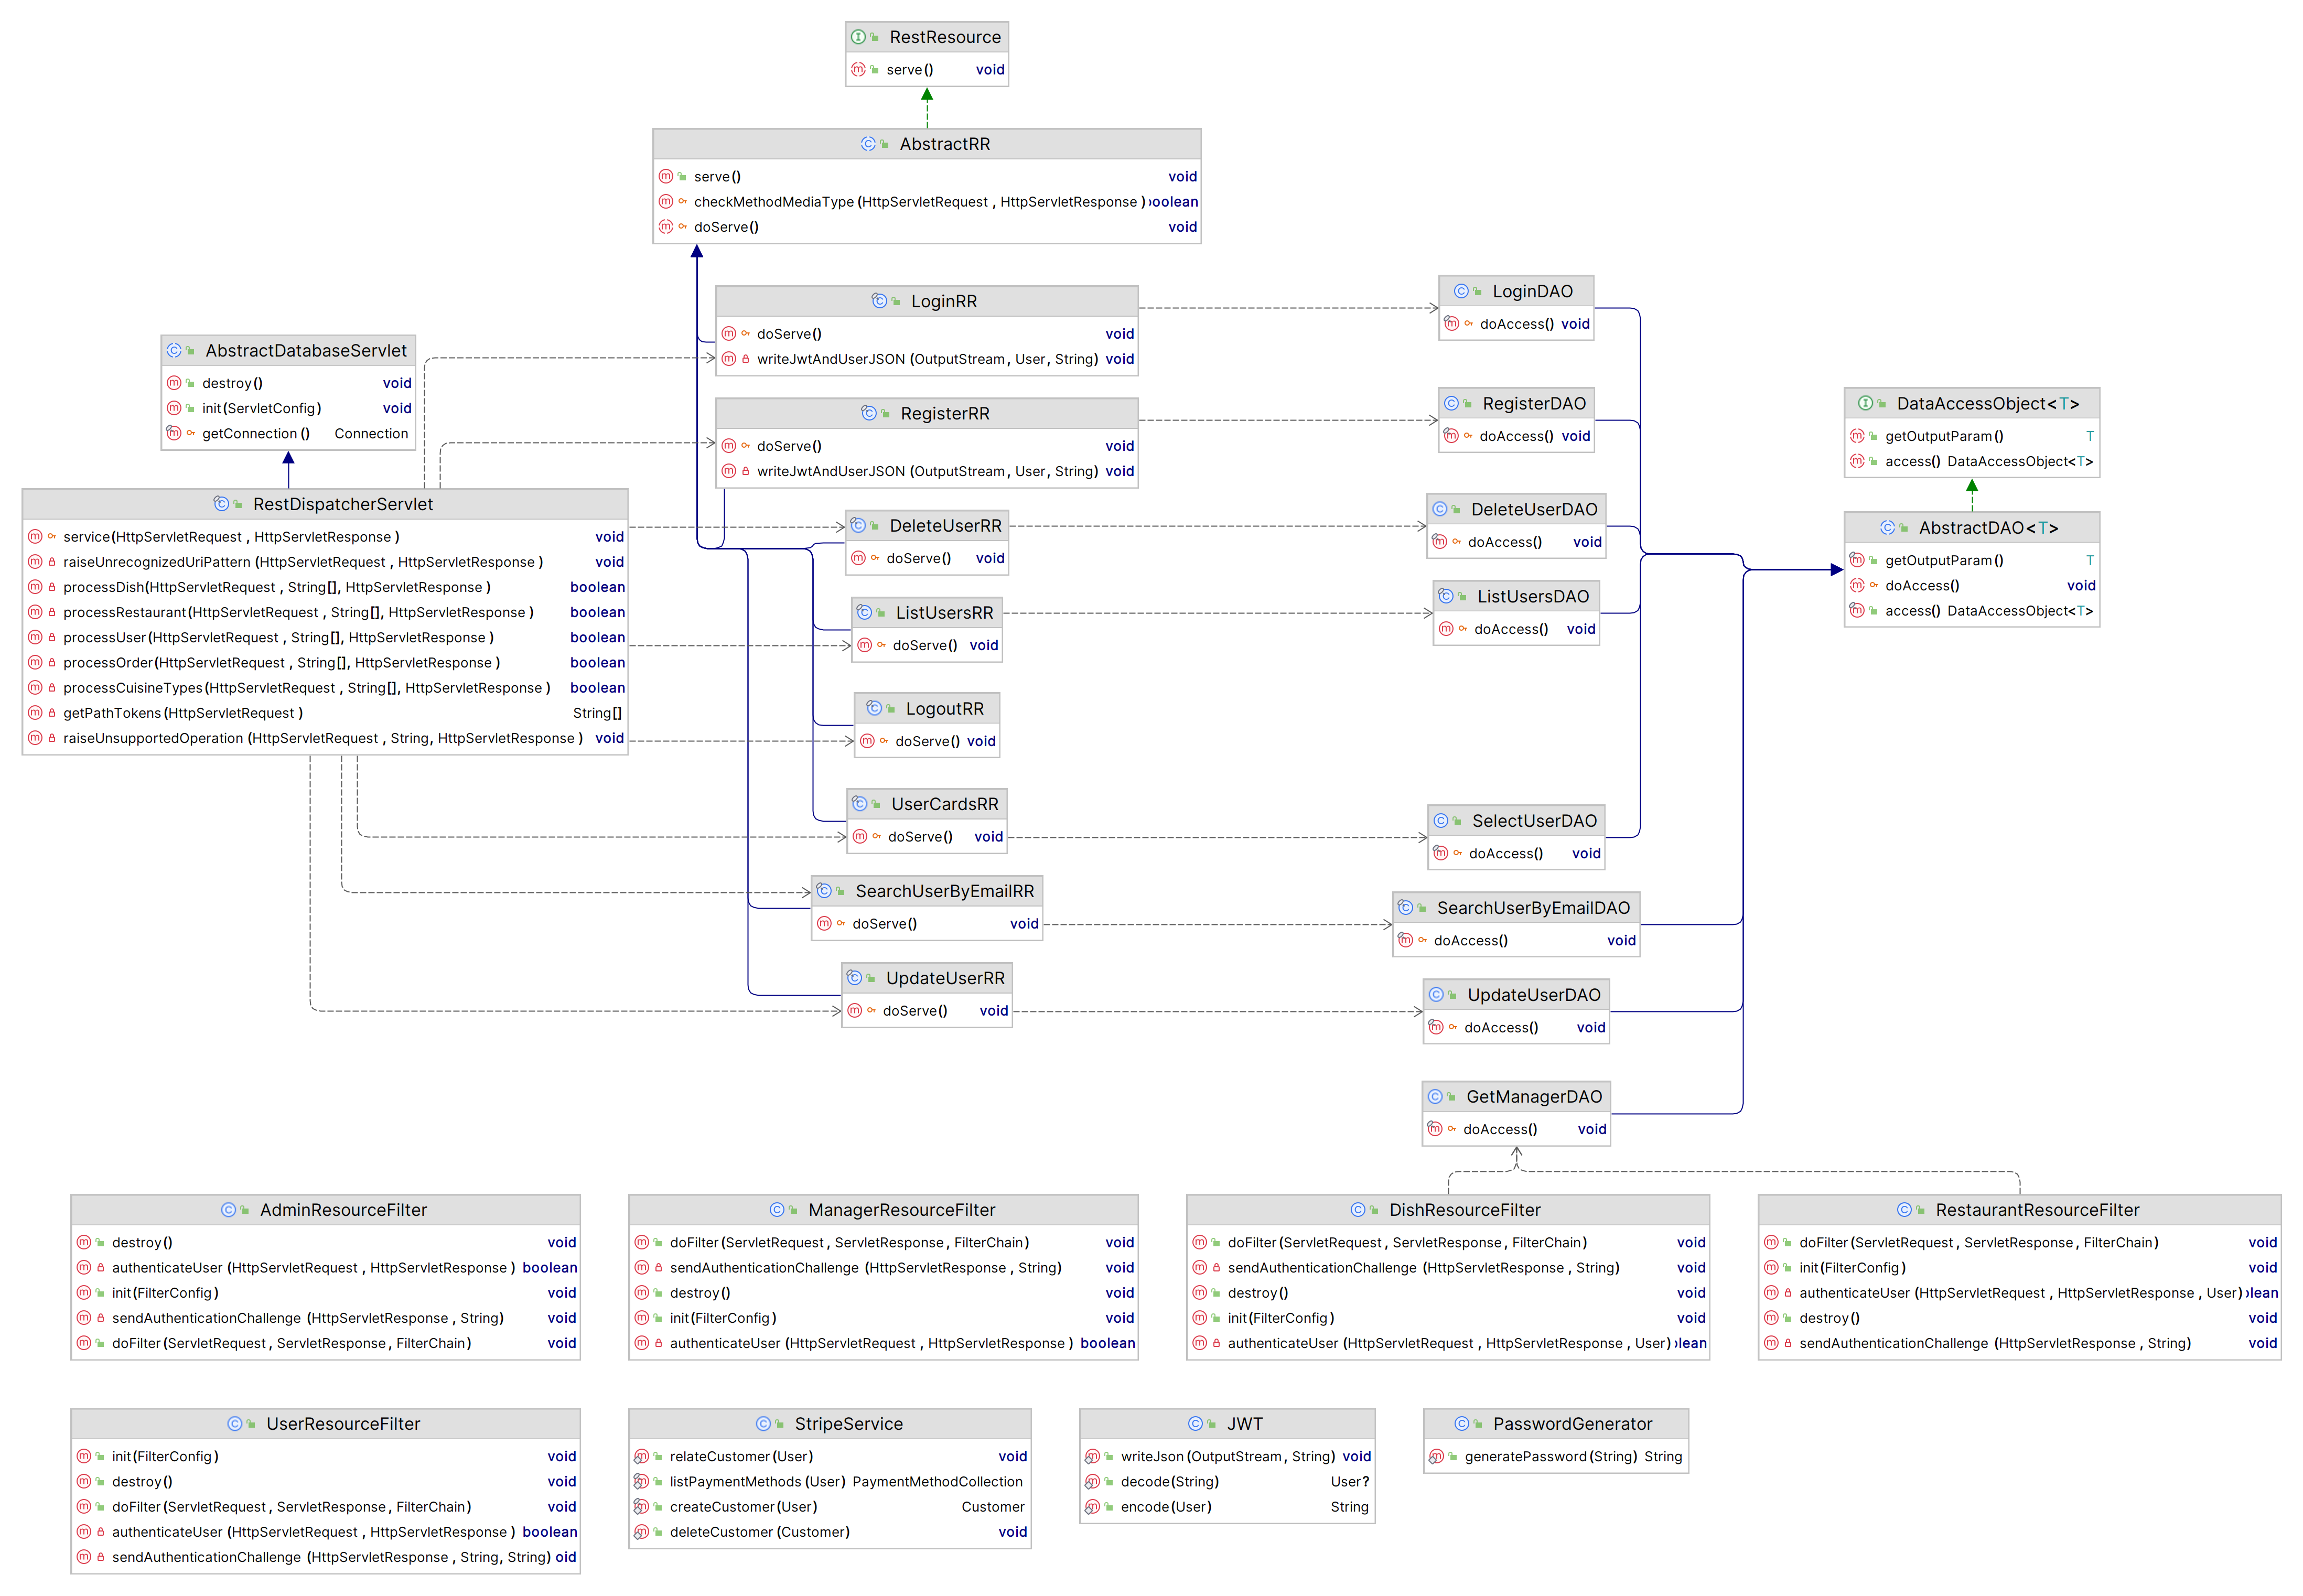
\includegraphics[width=1.0\textwidth]{resources/class-diagrams/user_class_diagram}
    \captionof{figure}{Class diagram of the user REST classes and the authentication filters.}
    \label{fig:class-user}
\end{center}


%Class diagram of the restaurant REST classes
\begin{center}
    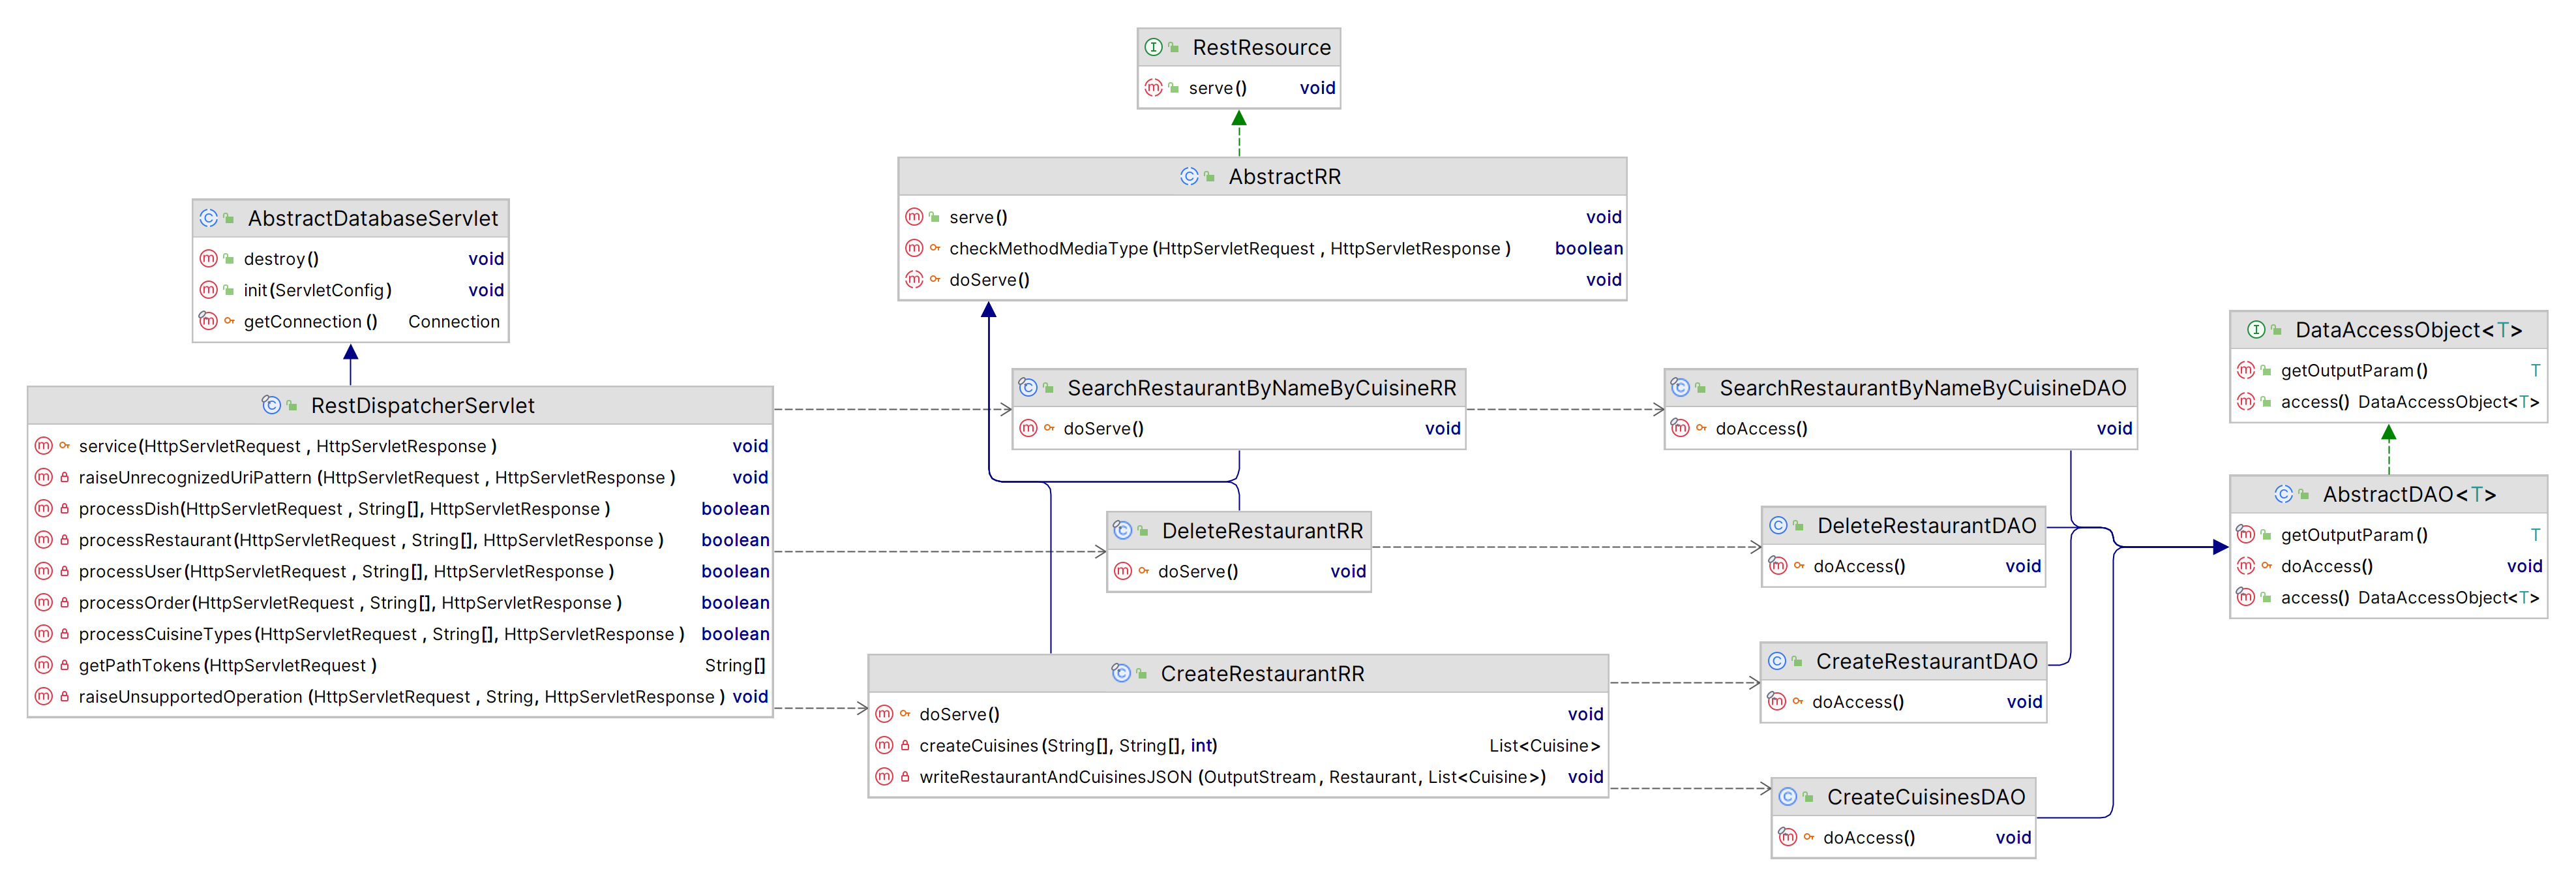
\includegraphics[width=1.0\textwidth]{resources/class-diagrams/restaurant_class_diagram}
    \captionof{figure}{Class diagram of the restaurant REST classes.}
    \label{fig:class-restaurant}
\end{center}


%Class diagram of the dish REST classes
\begin{center}
    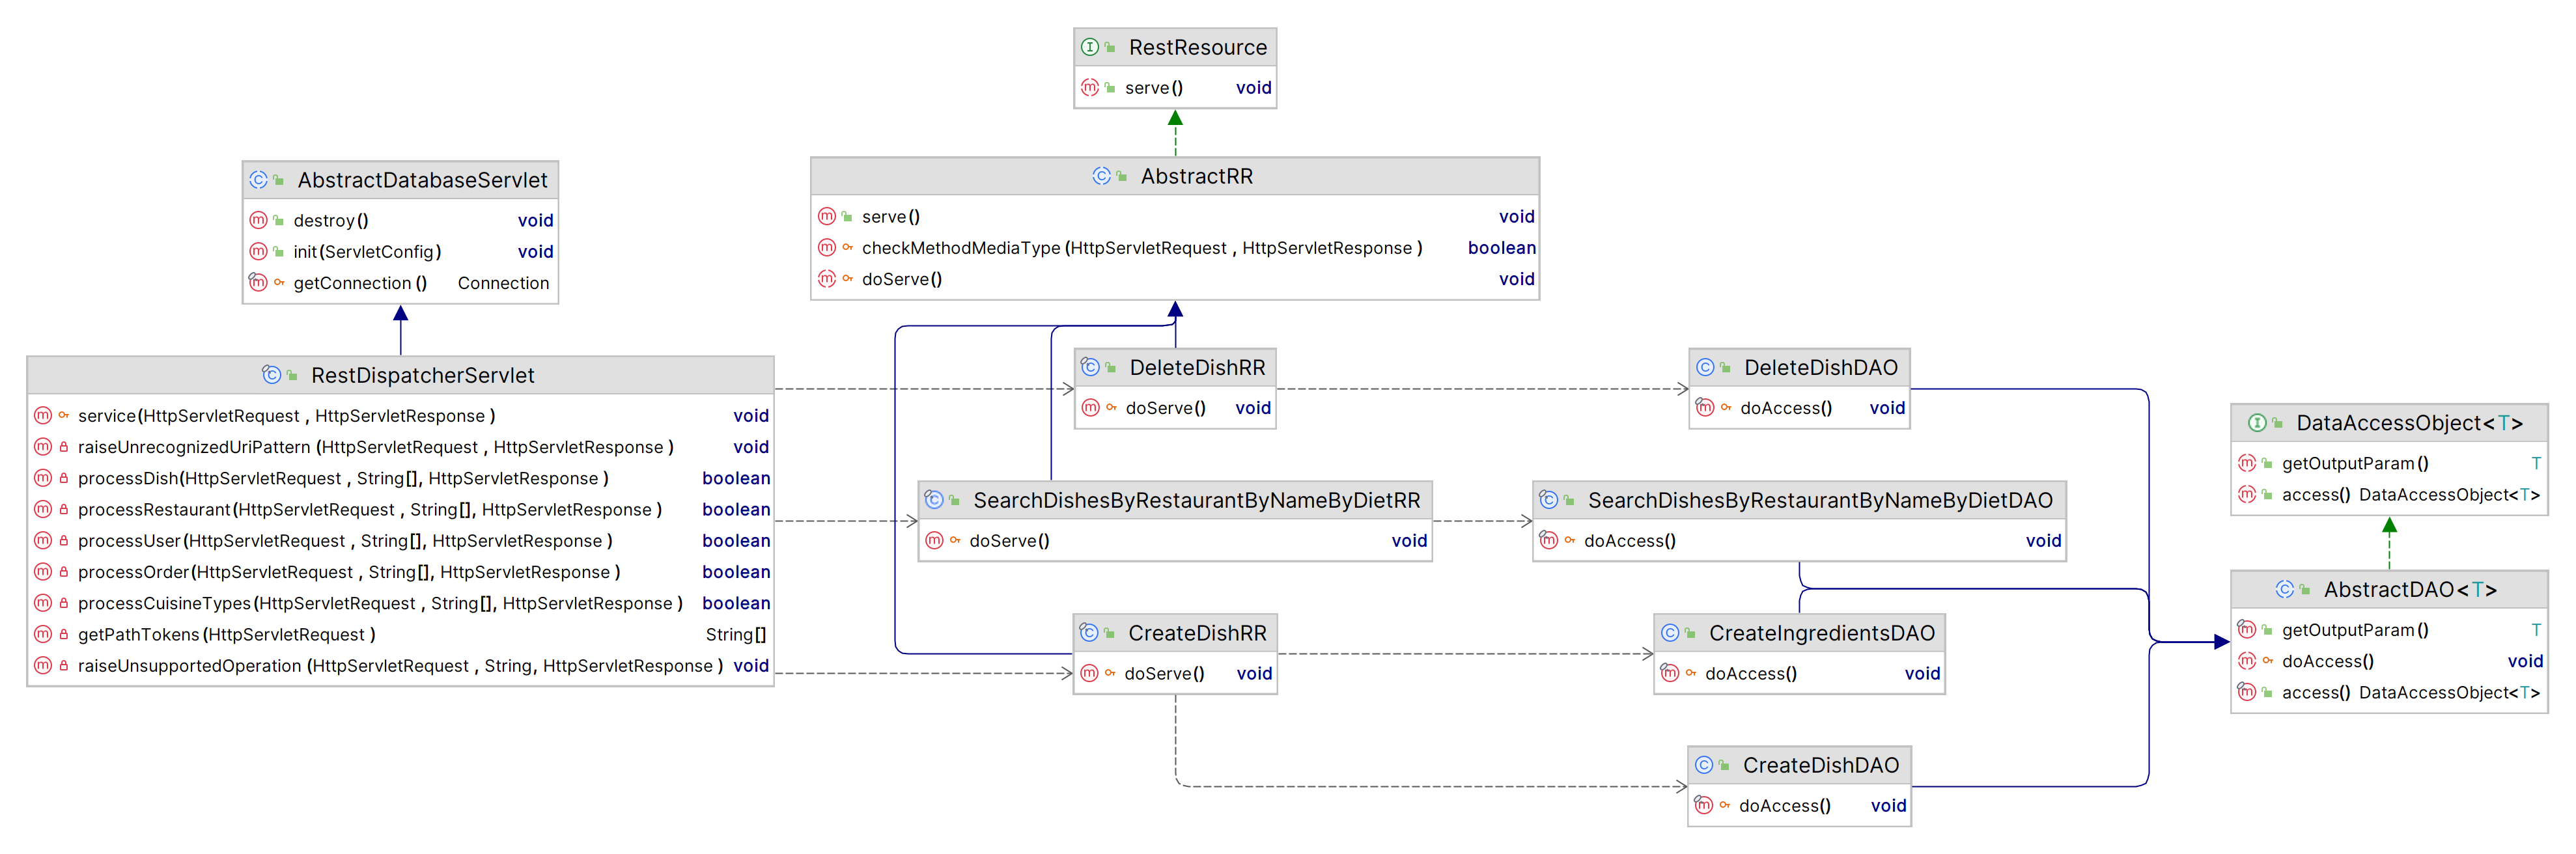
\includegraphics[width=1.0\textwidth]{resources/class-diagrams/dish_class_diagram}
    \captionof{figure}{Class diagram of the dish REST classes.}
    \label{fig:class-dish}
\end{center}


%Class diagram of the cuisine REST classes
\begin{center}
    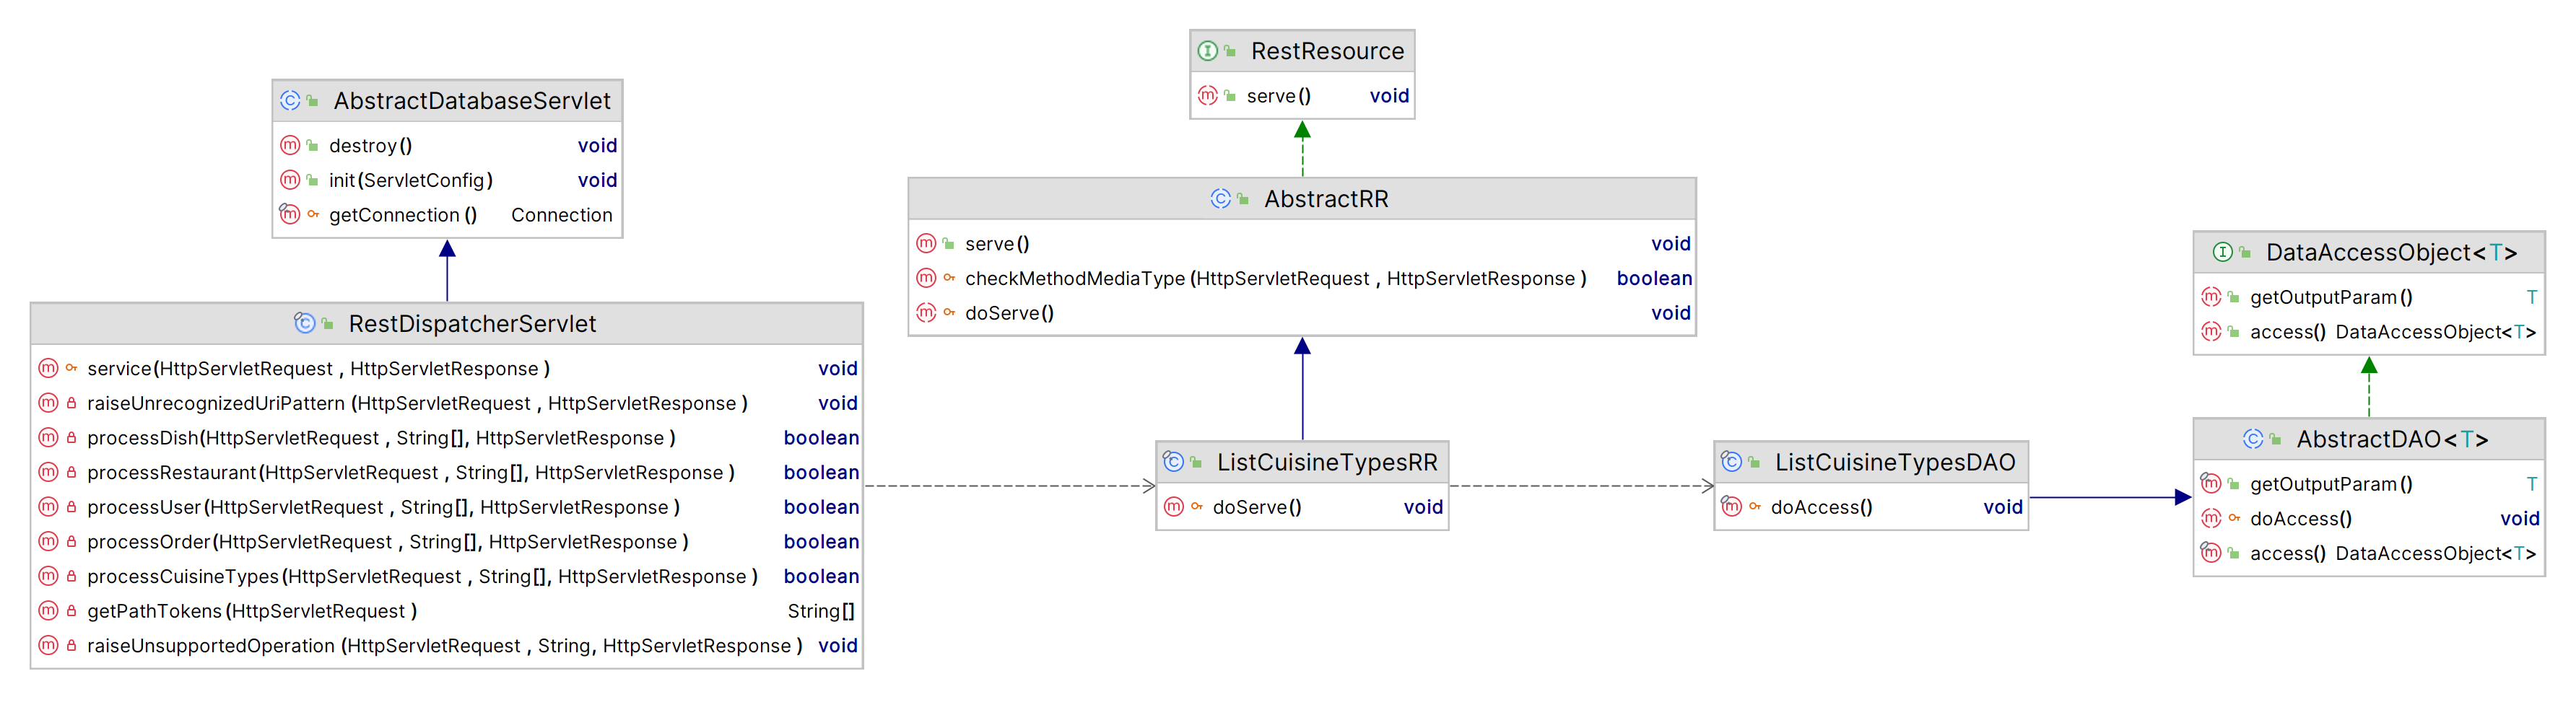
\includegraphics[width=1.0\textwidth]{resources/class-diagrams/cuisine_class_diagram}
    \captionof{figure}{Class diagram of the cuisine REST classes.}
    \label{fig:class-cuisine}
\end{center}


%Class diagram of the order REST classes
\begin{center}
    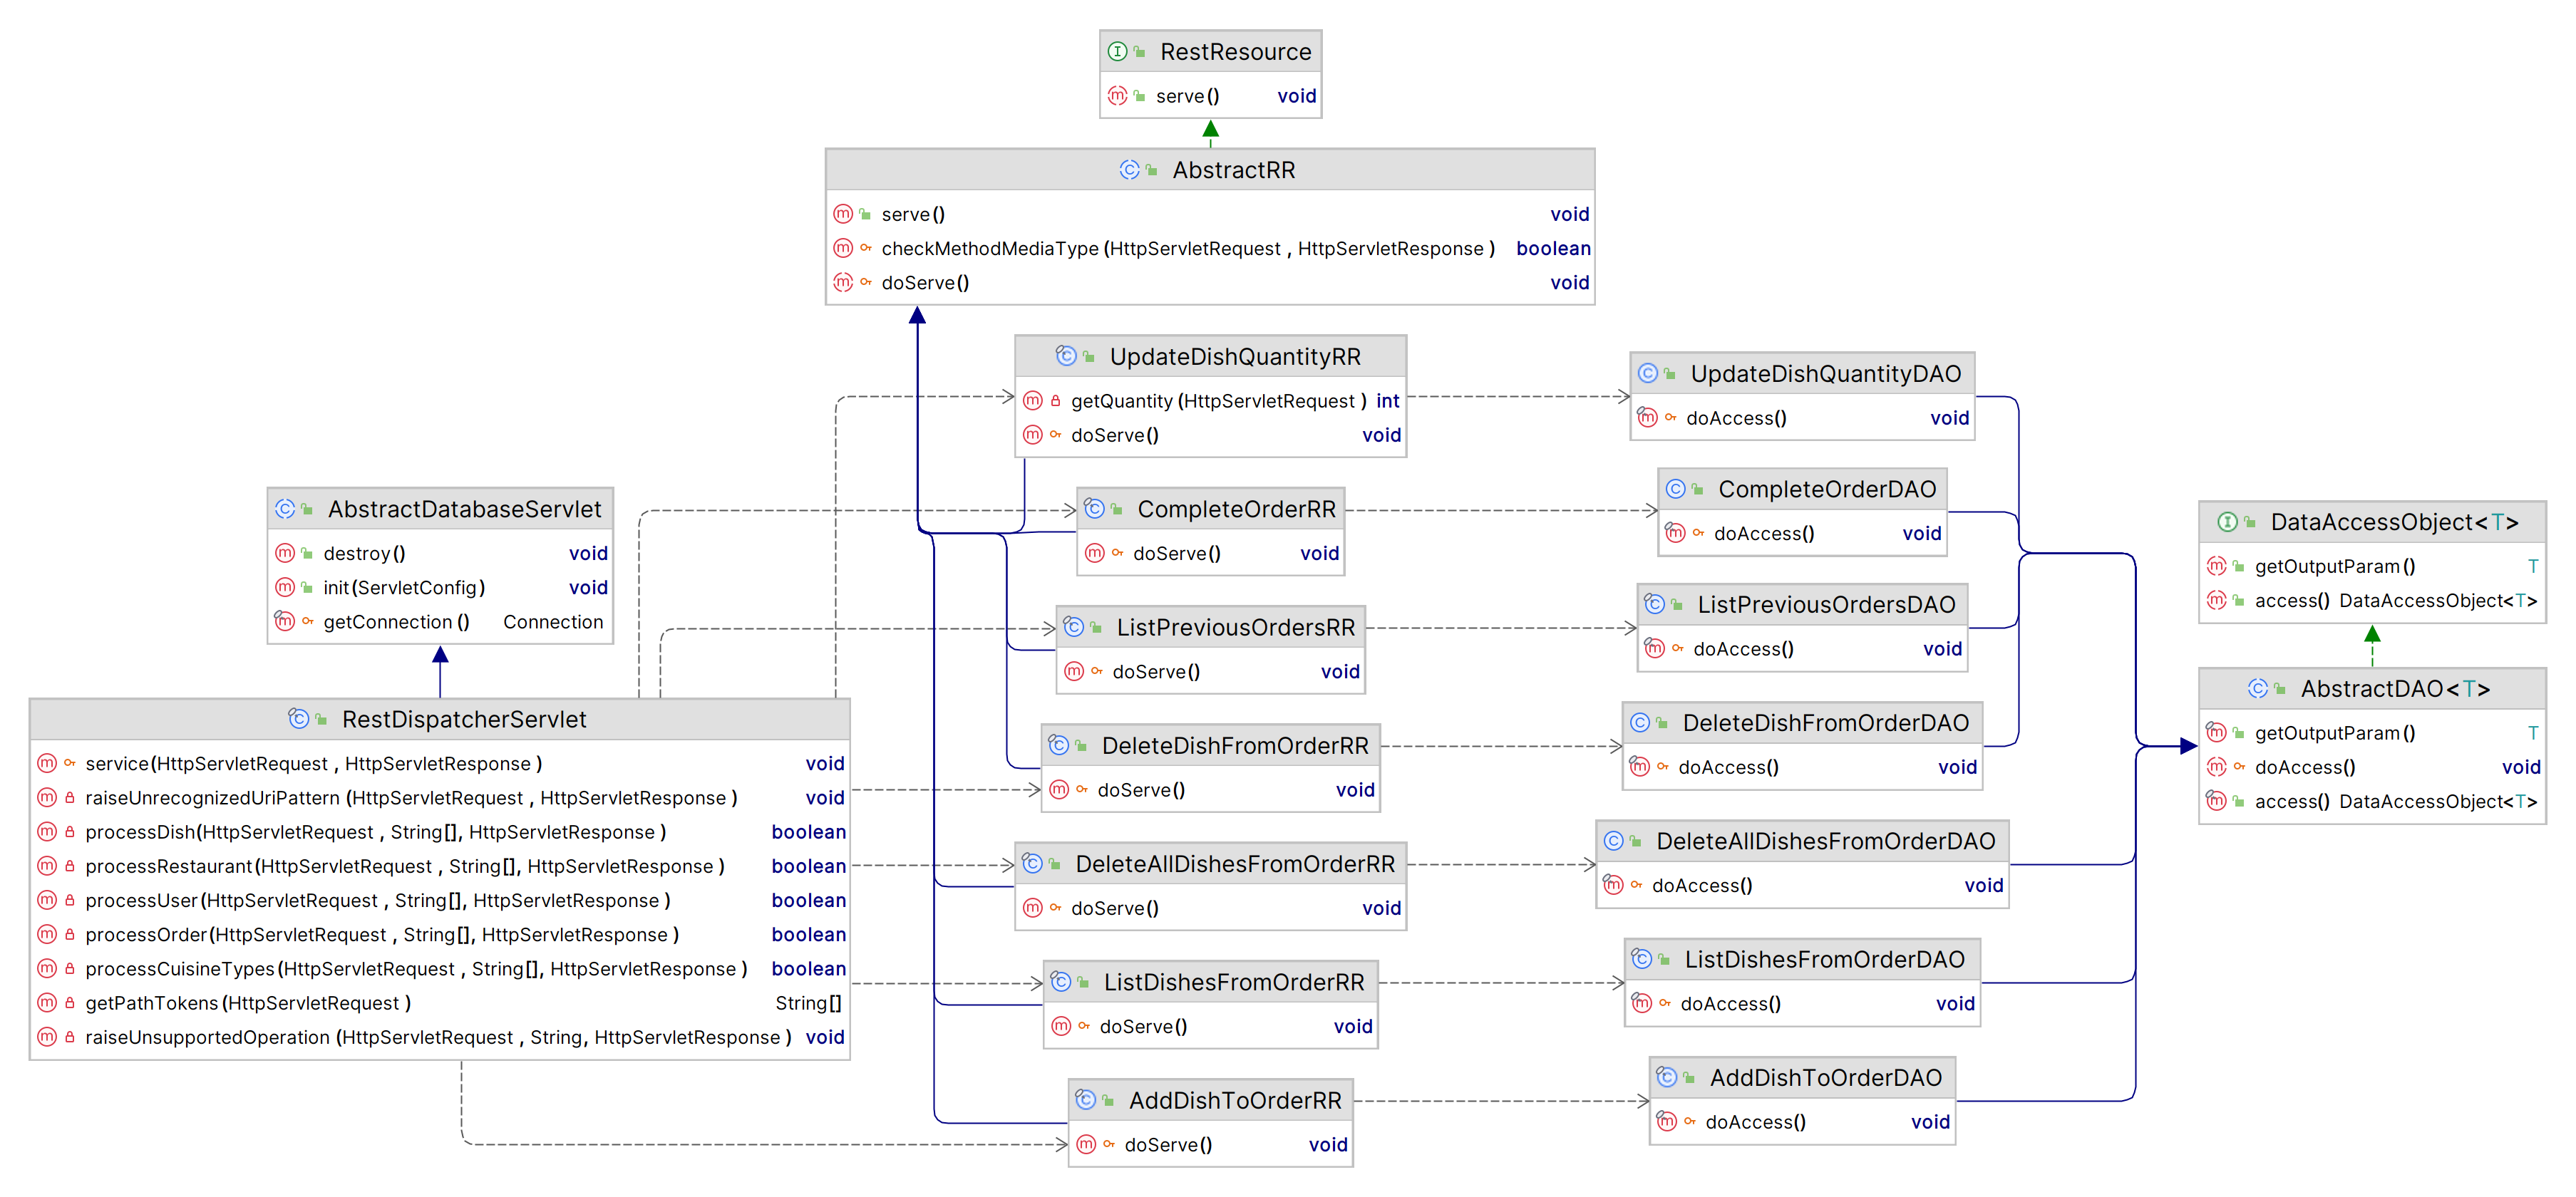
\includegraphics[width=1.0\textwidth]{resources/class-diagrams/order_class_diagram}
    \captionof{figure}{Class diagram of the order REST classes.}
    \label{fig:class-order}
\end{center}

%Go to a new page before next section (leaves space for the images)
\newpage
